% \chapter{Implementation}
\chapter{Implementation}
In this chapter, we present the process of implementing the system. Up to the end of the Specialized Project, we have completed the following tasks:
\begin{itemize}
    \item Designed a mockup interface for the website.
    \item Developed a crawler to collect data from both real estate websites and Facebook groups.
    \item Developed an intent classification model to classify the user's intent based on the user's message.
\end{itemize}

\section{Mockup interface}
We have implemented the mockup interface in Figma for the Tenant Landing Page, Search page, Rental detail page and Chatbot interface.

\subsection{Tenant pages}
We have a tenant landing page that allows the user to view the list of rental posts in the system. You can see the design in Figure \ref{fig:tenant-landing-page}

\clearpage
\begin{figure}[ht]
    \centering
    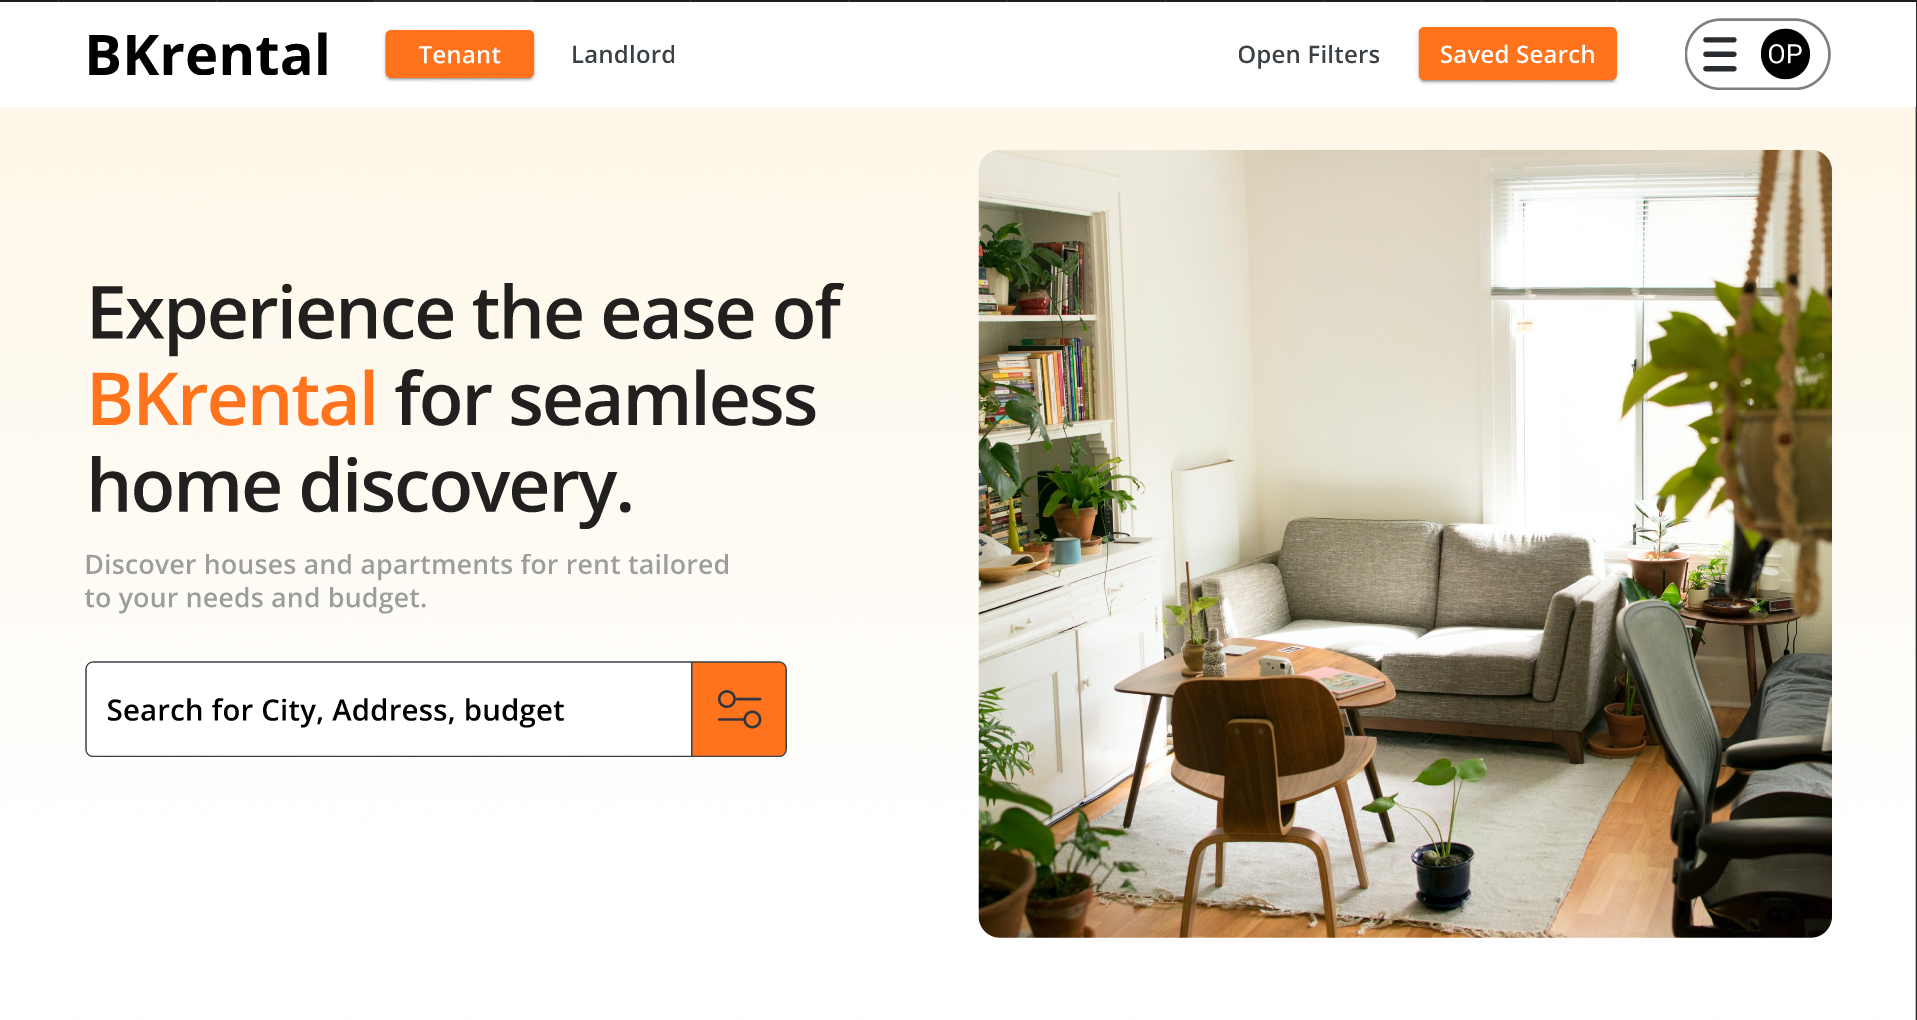
\includegraphics[width=0.8\textwidth]{Images/Mockup/landing_page.png}
    \caption{The tenant landing page}
    \label{fig:tenant-landing-page}
\end{figure}

The list of rental posts is displayed in the form of a card, see Figure \ref{fig:rental-posts}

\begin{figure}[ht]
    \centering
    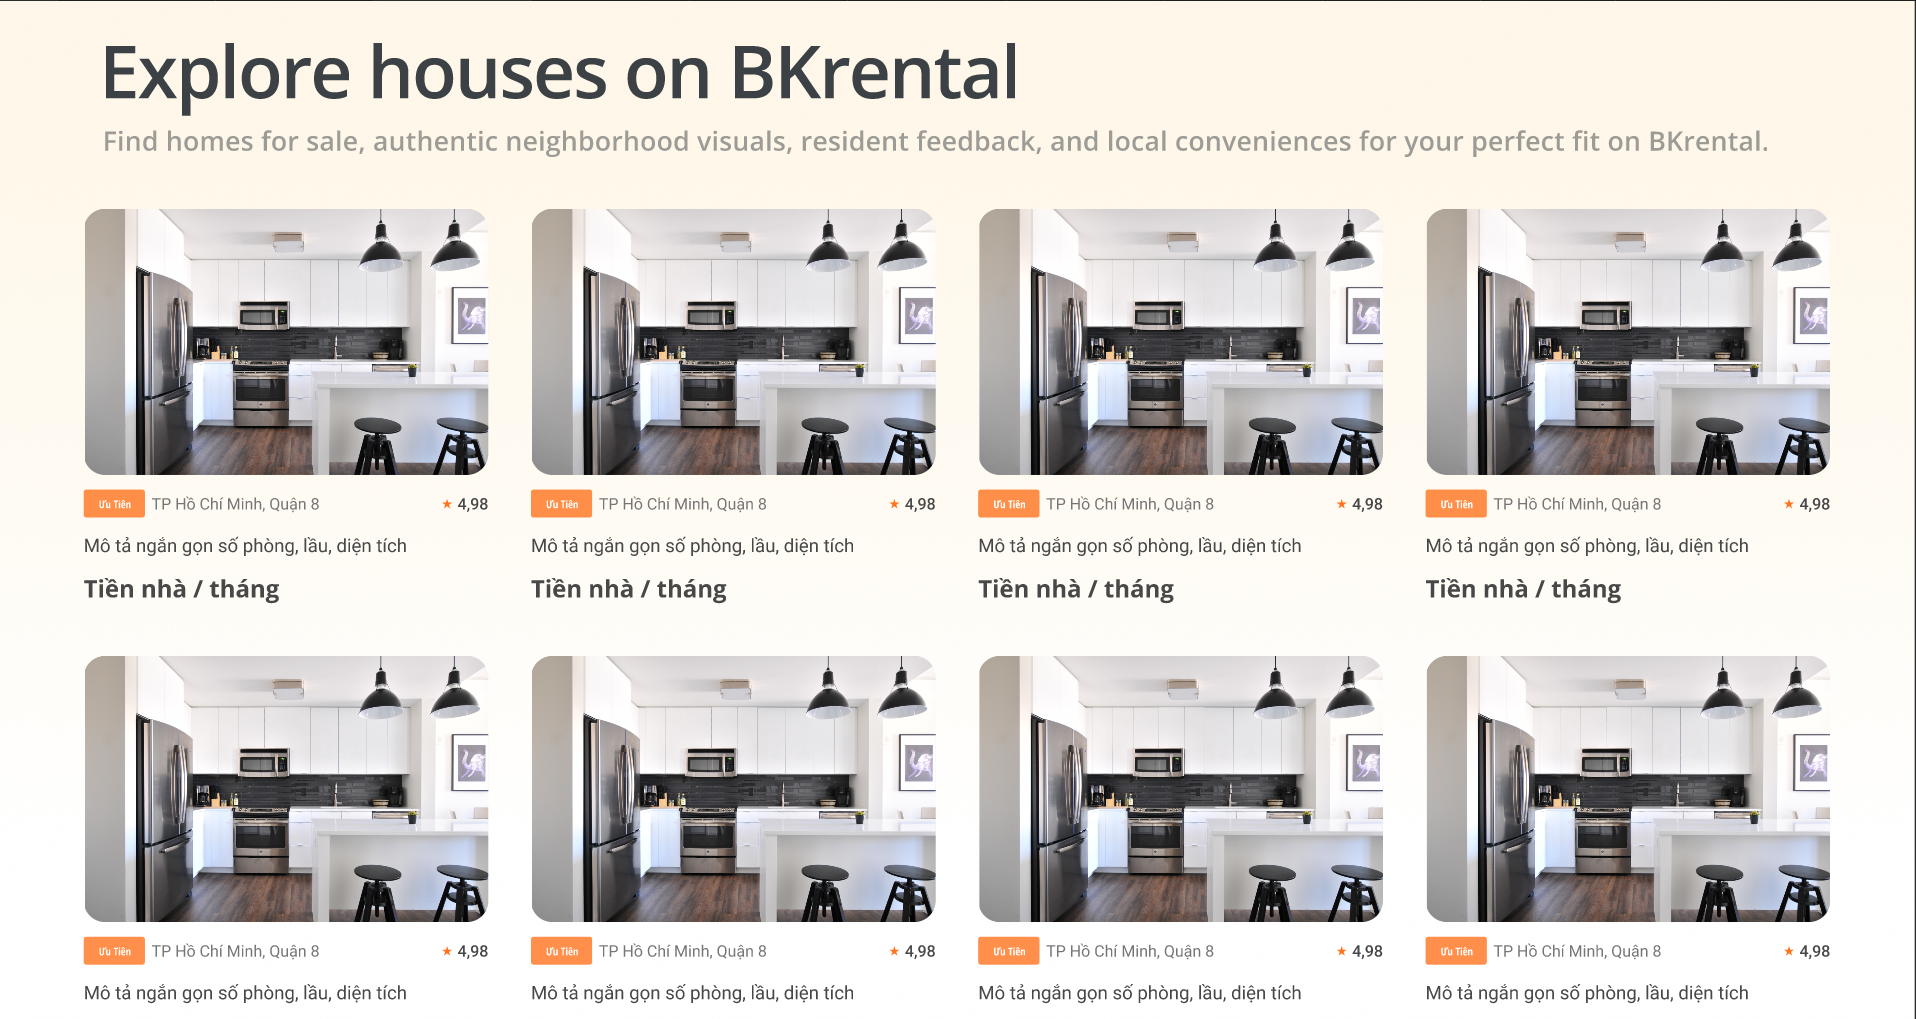
\includegraphics[width=0.8\textwidth]{Images/Mockup/rental_posts.png}
    \caption{The list of rental posts}
    \label{fig:rental-posts} 
\end{figure}

When the user clicks on a rental post, the rental detail page will be displayed. The rental detail page contains the information of the rental post such as the name, address, price, area, description, owner name, owner contact, post date, and the link to the original post. The rental detail page is shown in Figures \ref{fig:rental-detail-page} and \ref{fig:rental-detail-page-2}

\begin{figure}[ht]
    \centering
    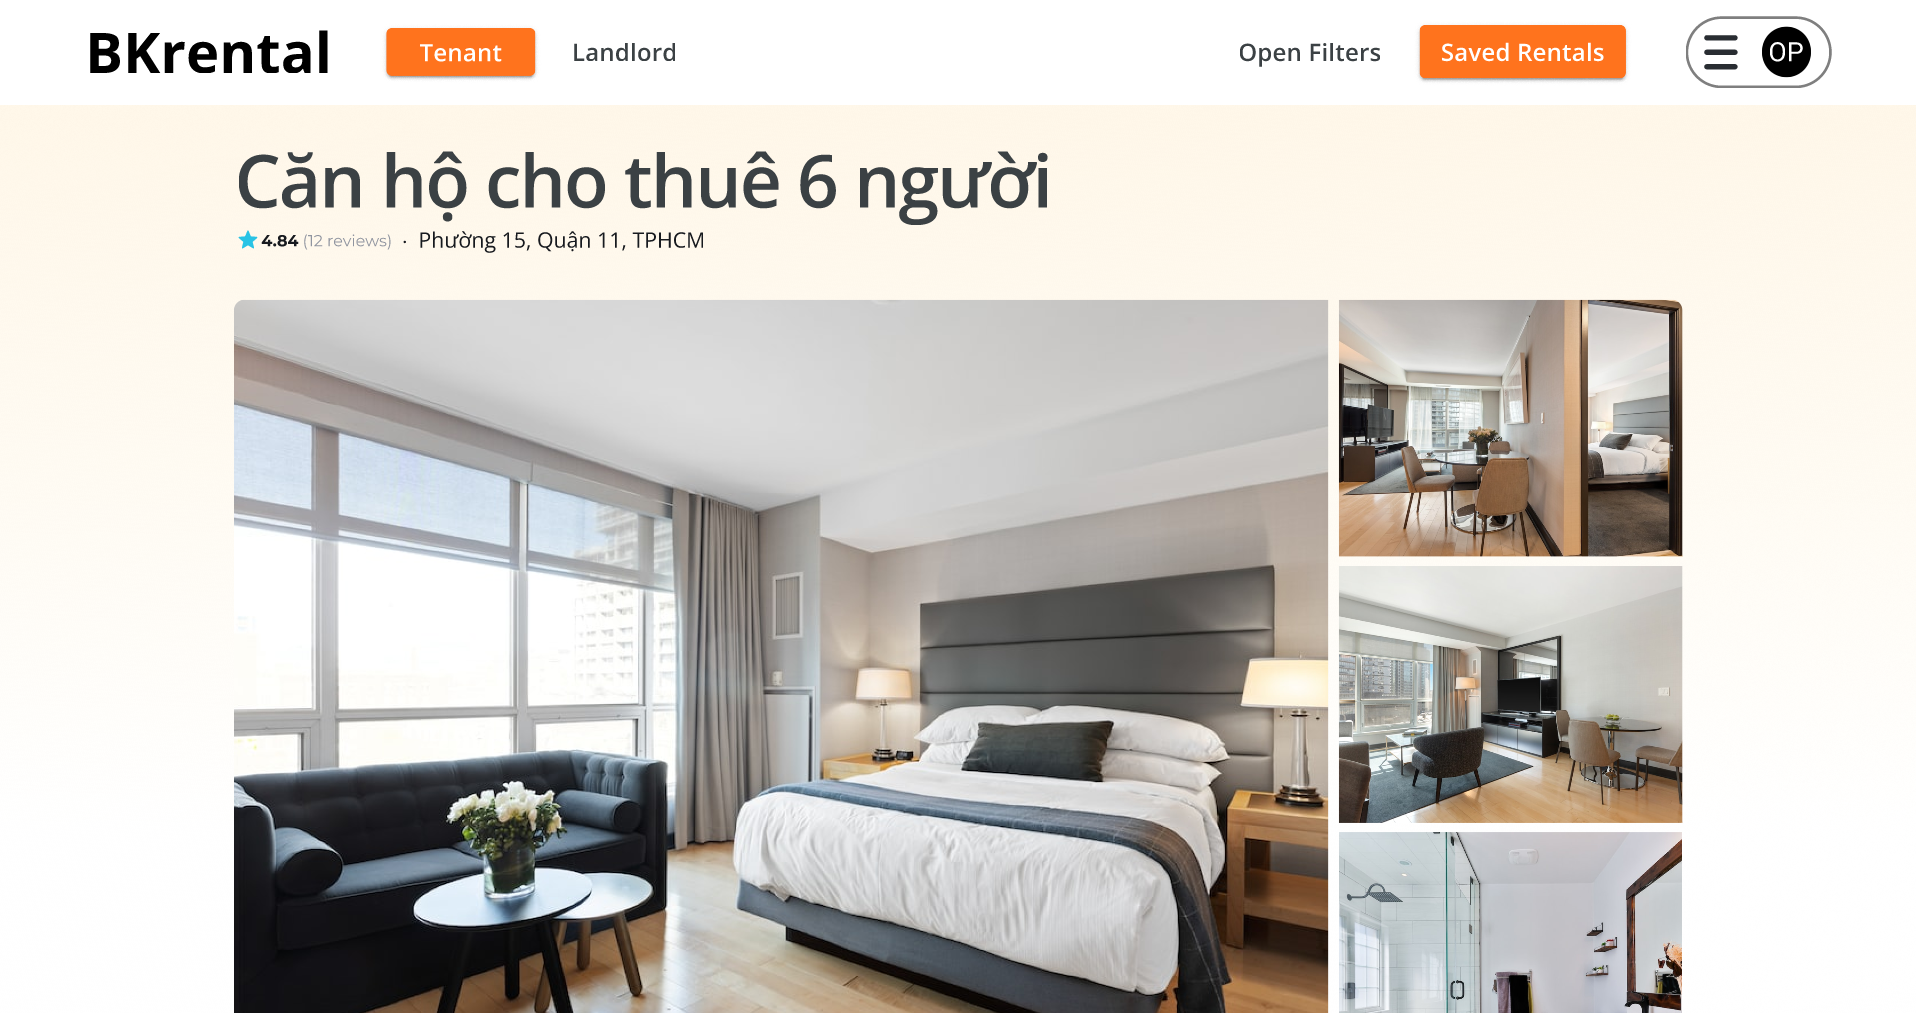
\includegraphics[width=\textwidth]{Images/Mockup/rental_detail_1.png}
    \caption{The rental detail page}
    \label{fig:rental-detail-page}
\end{figure}

\begin{figure}[ht]
    \centering
    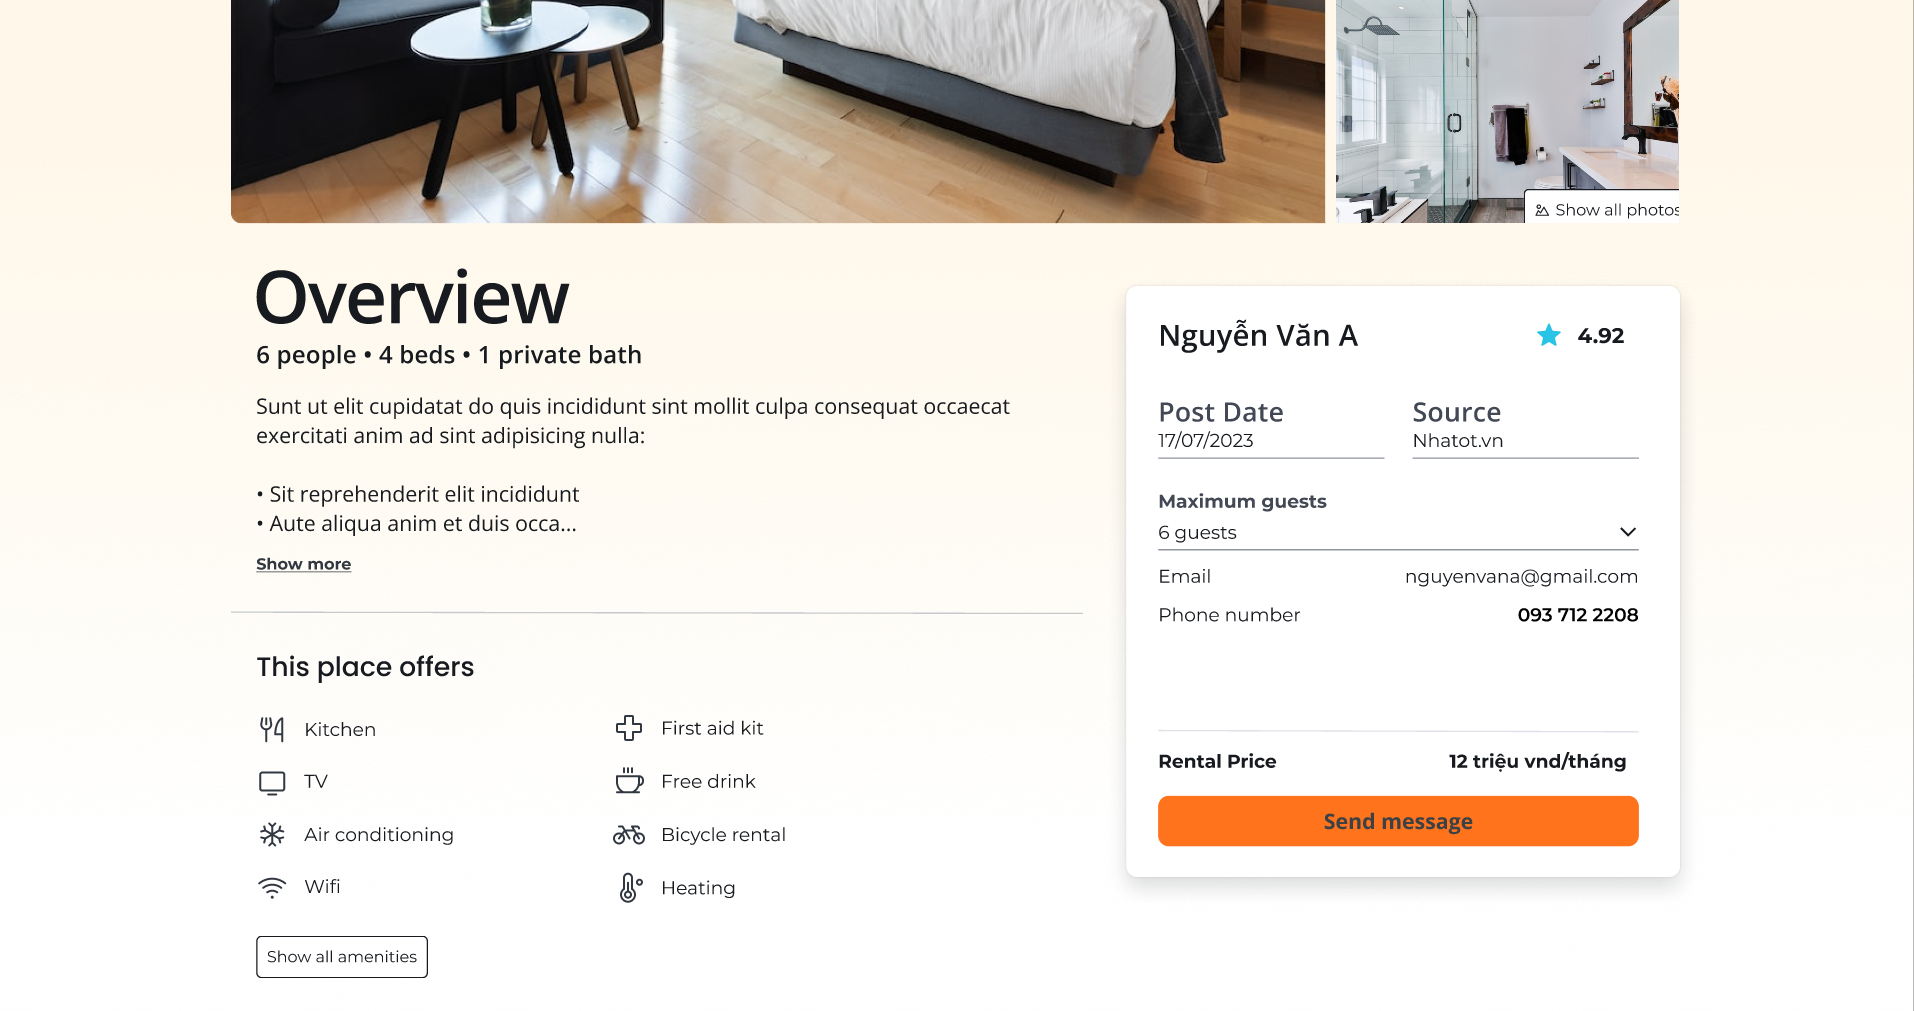
\includegraphics[width=\textwidth]{Images/Mockup/rental_detail_2.png}
    \caption{The rental detail page (continue)}
    \label{fig:rental-detail-page-2}
\end{figure}
\clearpage

\subsection{Search and Filter page}
Our website allows the user to search by keyword and filter the rental posts by some criteria such as property type, price range, number of rooms, number of beds, area and amenities. 

\begin{figure}[ht]
    \centering
    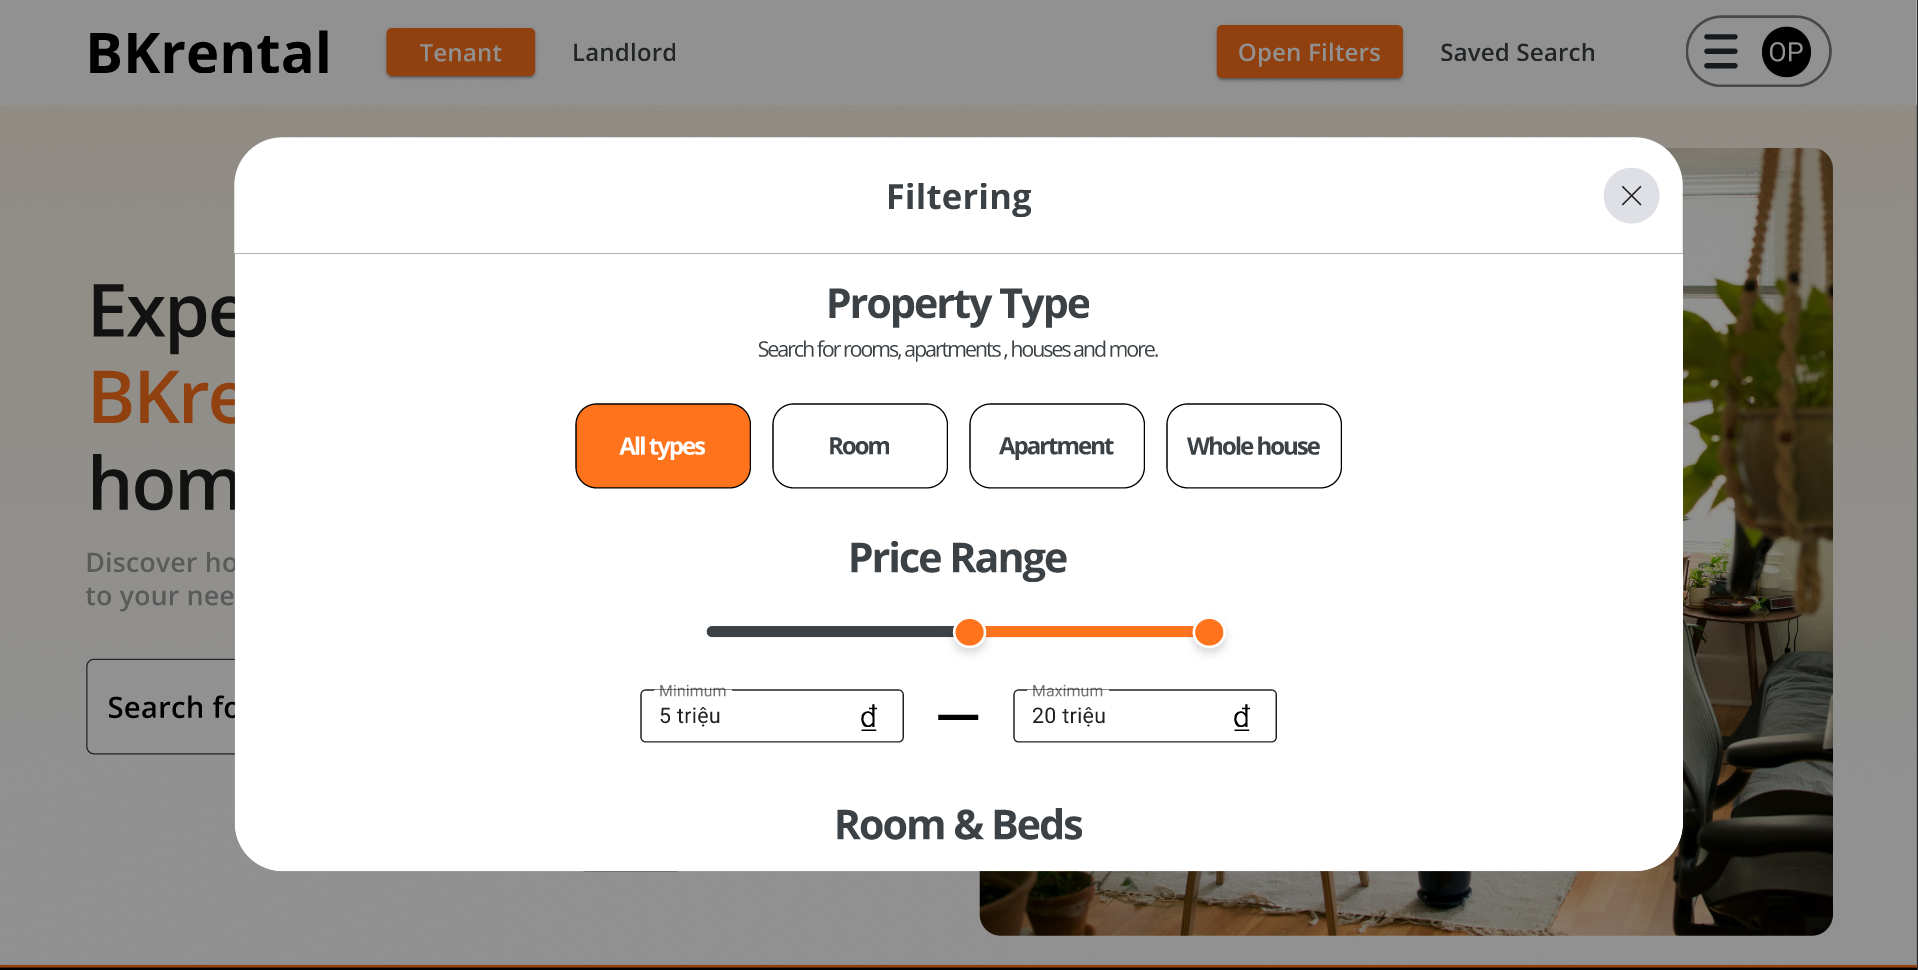
\includegraphics[width=\textwidth]{Images/Mockup/rental_filter_1.png}
    \caption{The rental filter page}
    \label{fig:rental-filter-1} 
\end{figure}

\begin{figure}[ht]
    \centering
    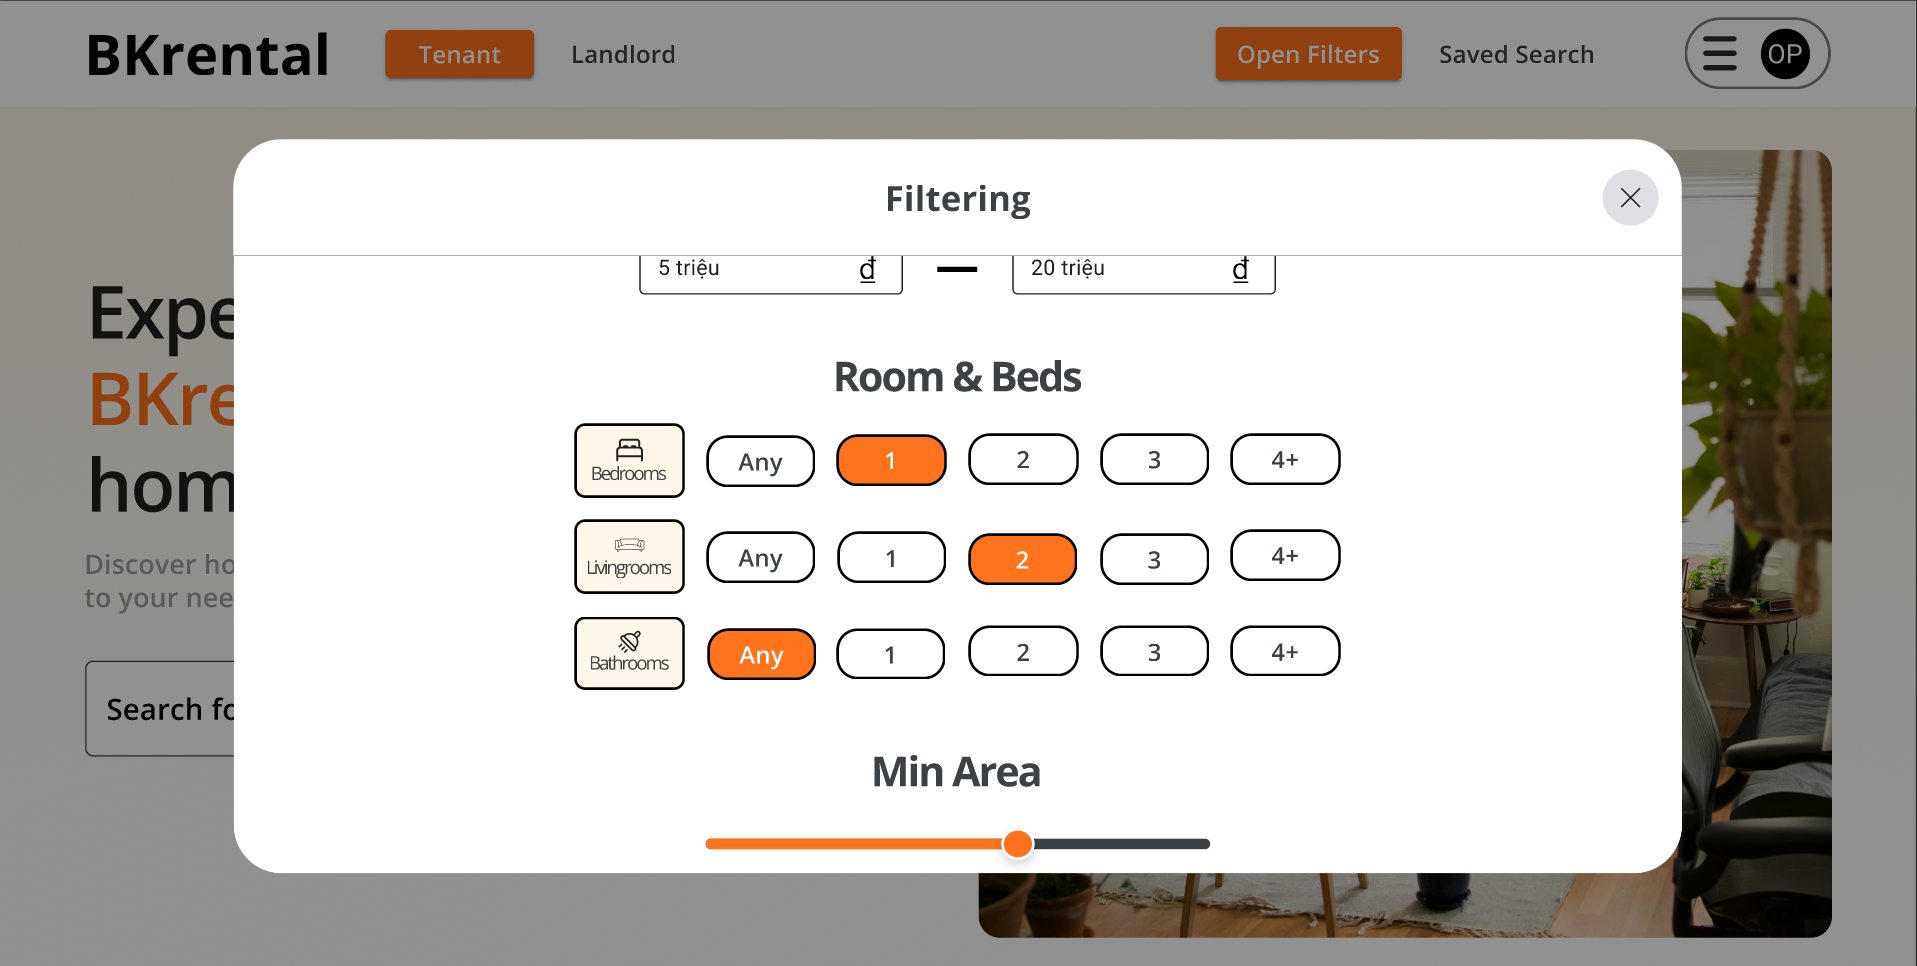
\includegraphics[width=\textwidth]{Images/Mockup/rental_filter_2.png}
    \caption{The rental filter page (continue)}
    \label{fig:rental-filter-2} 
\end{figure}

\begin{figure}[ht]
    \centering
    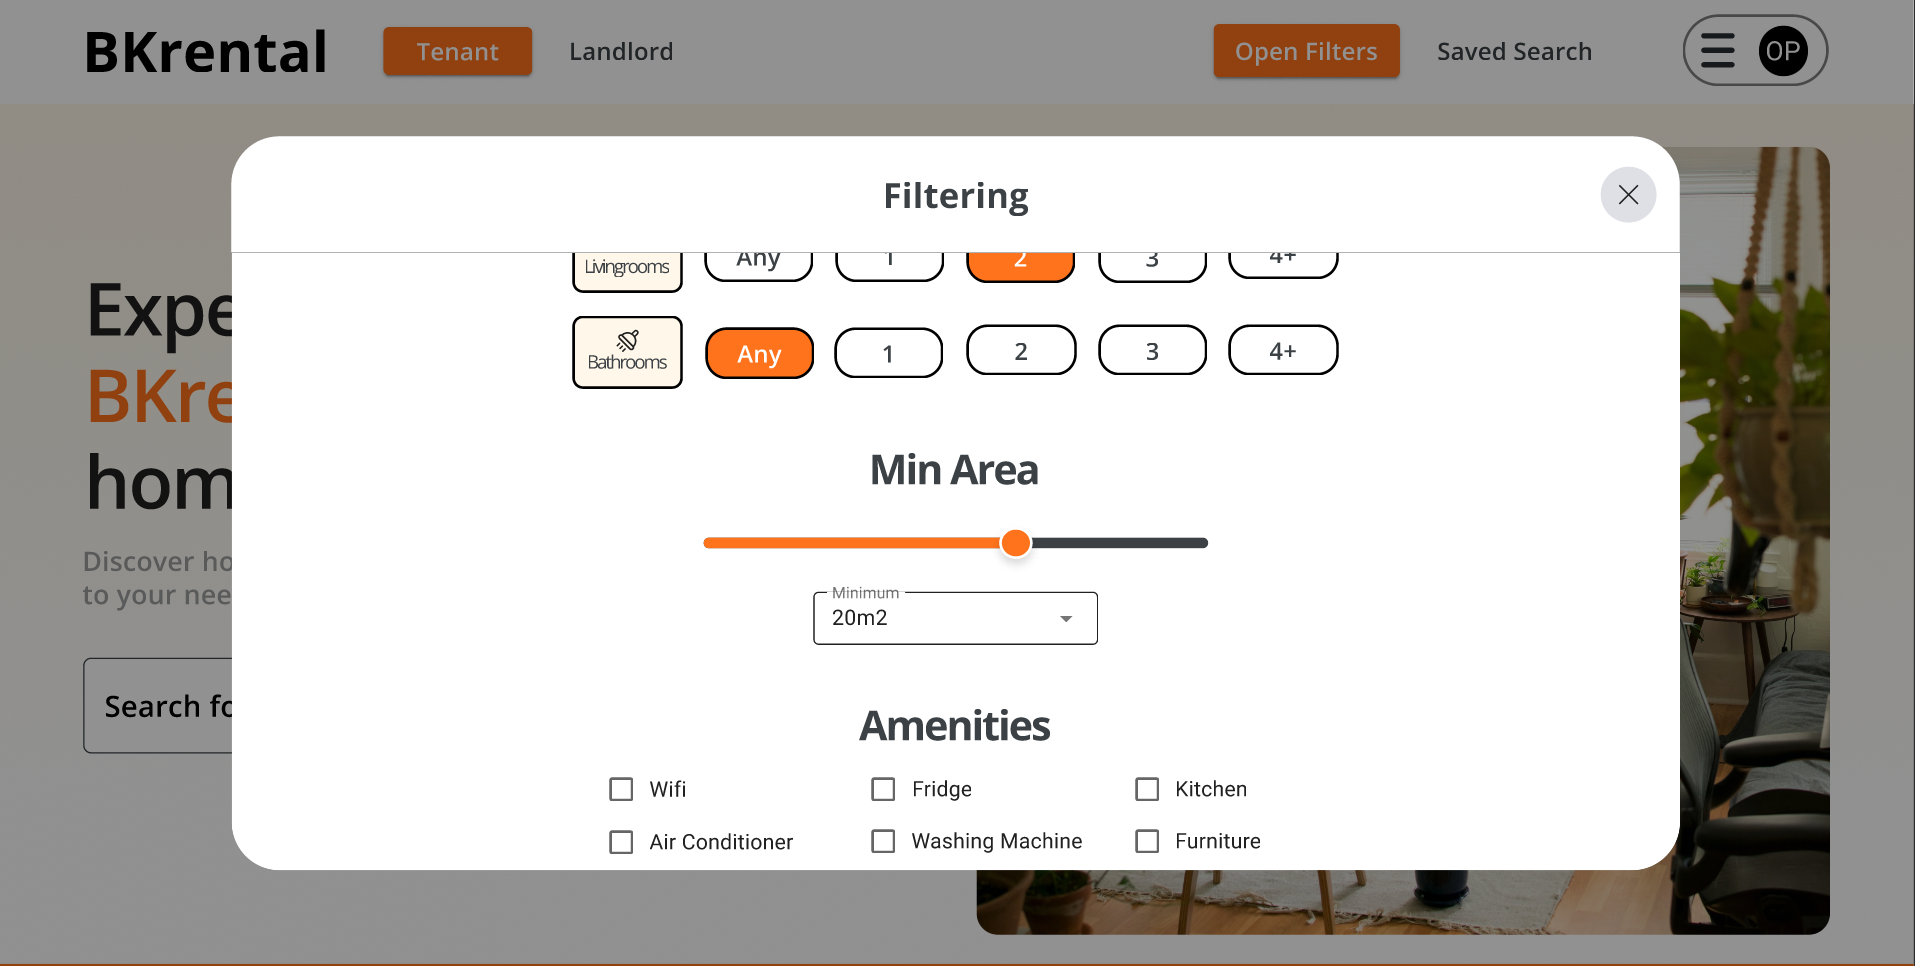
\includegraphics[width=\textwidth]{Images/Mockup/rental_filter_3.png}
    \caption{The rental filter page (continue)}
    \label{fig:rental-filter-3} 
\end{figure}

\clearpage

\subsection{Chatbot interface}

\begin{figure}[ht]
    \centering
    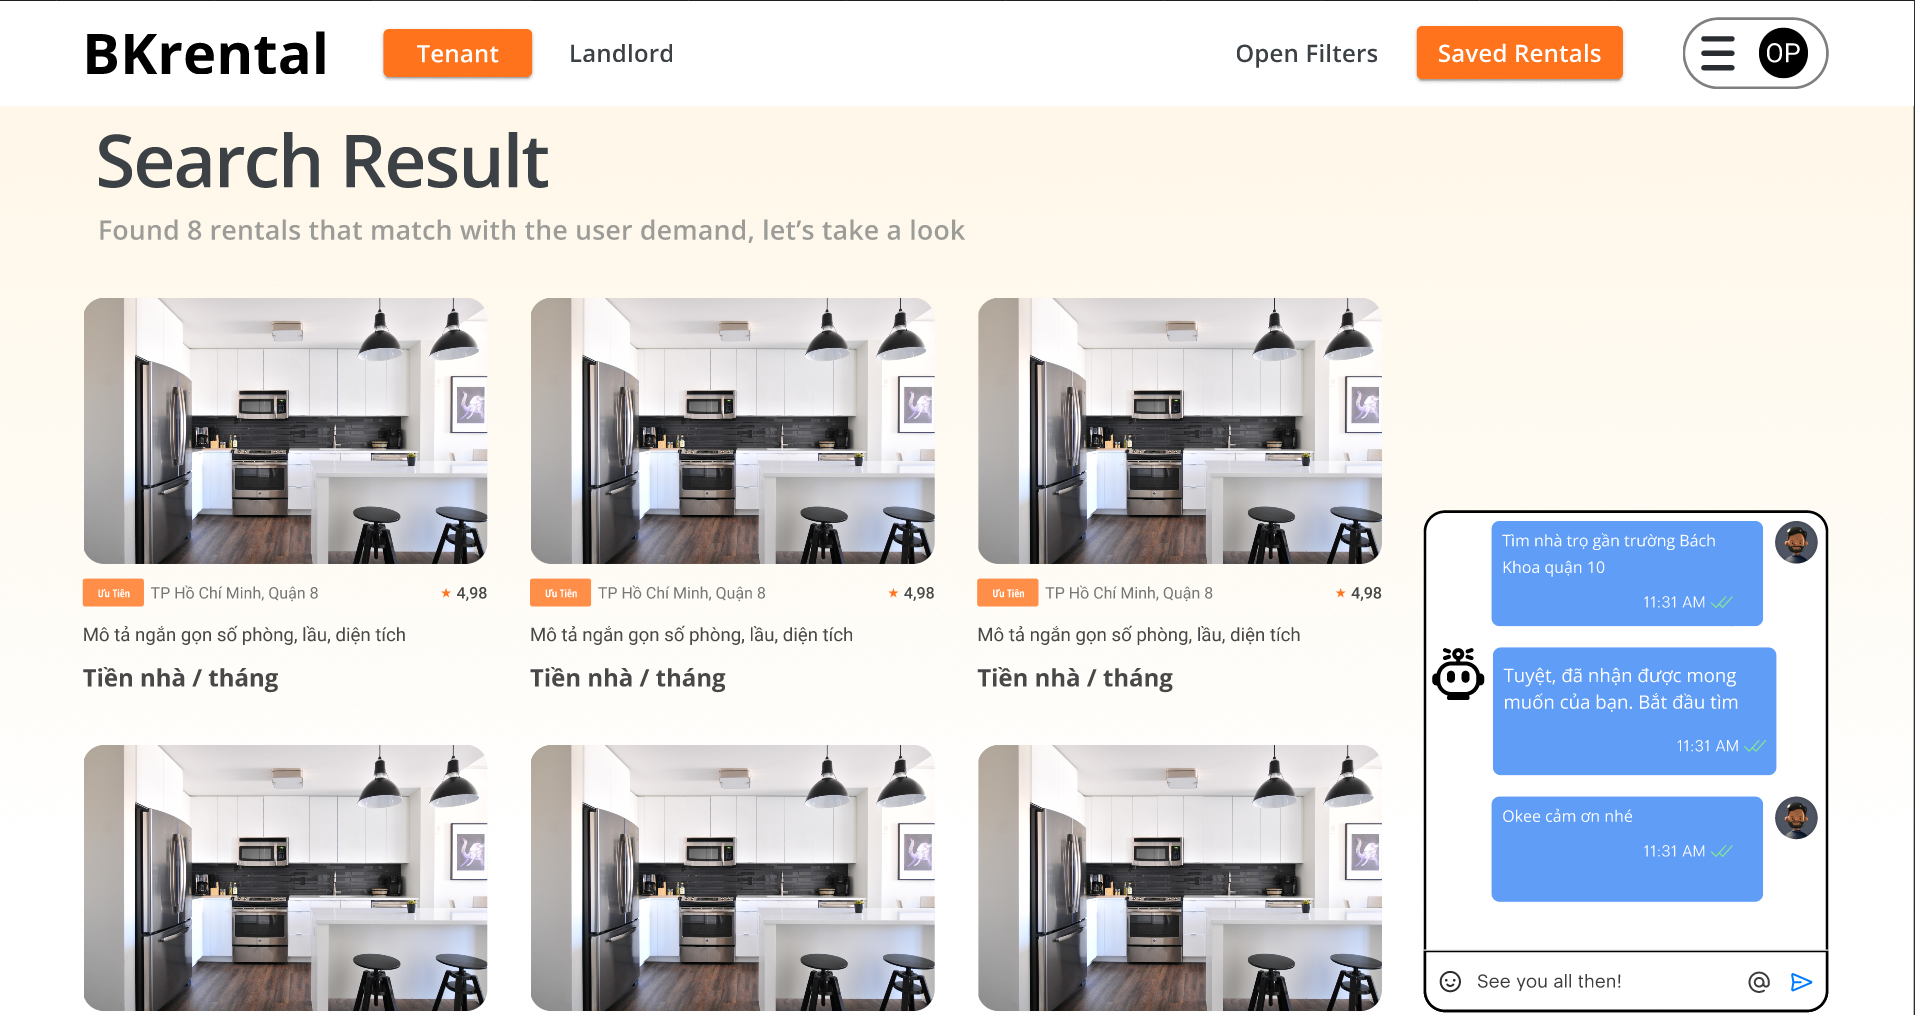
\includegraphics[width=\textwidth]{Images/Mockup/chatbot.png}
    \caption{The chatbot interface}
    \label{fig:chatbot}
\end{figure}

\clearpage

\subsection{Landlord pages}
We have landlord pages that allow the landlord to post their rental information and manage their property. Figures \ref{fig:create-rental-1} and \ref{fig:create-rental-2} show the form for the landlord to create a new rental post

\begin{figure}[ht]
    \centering
    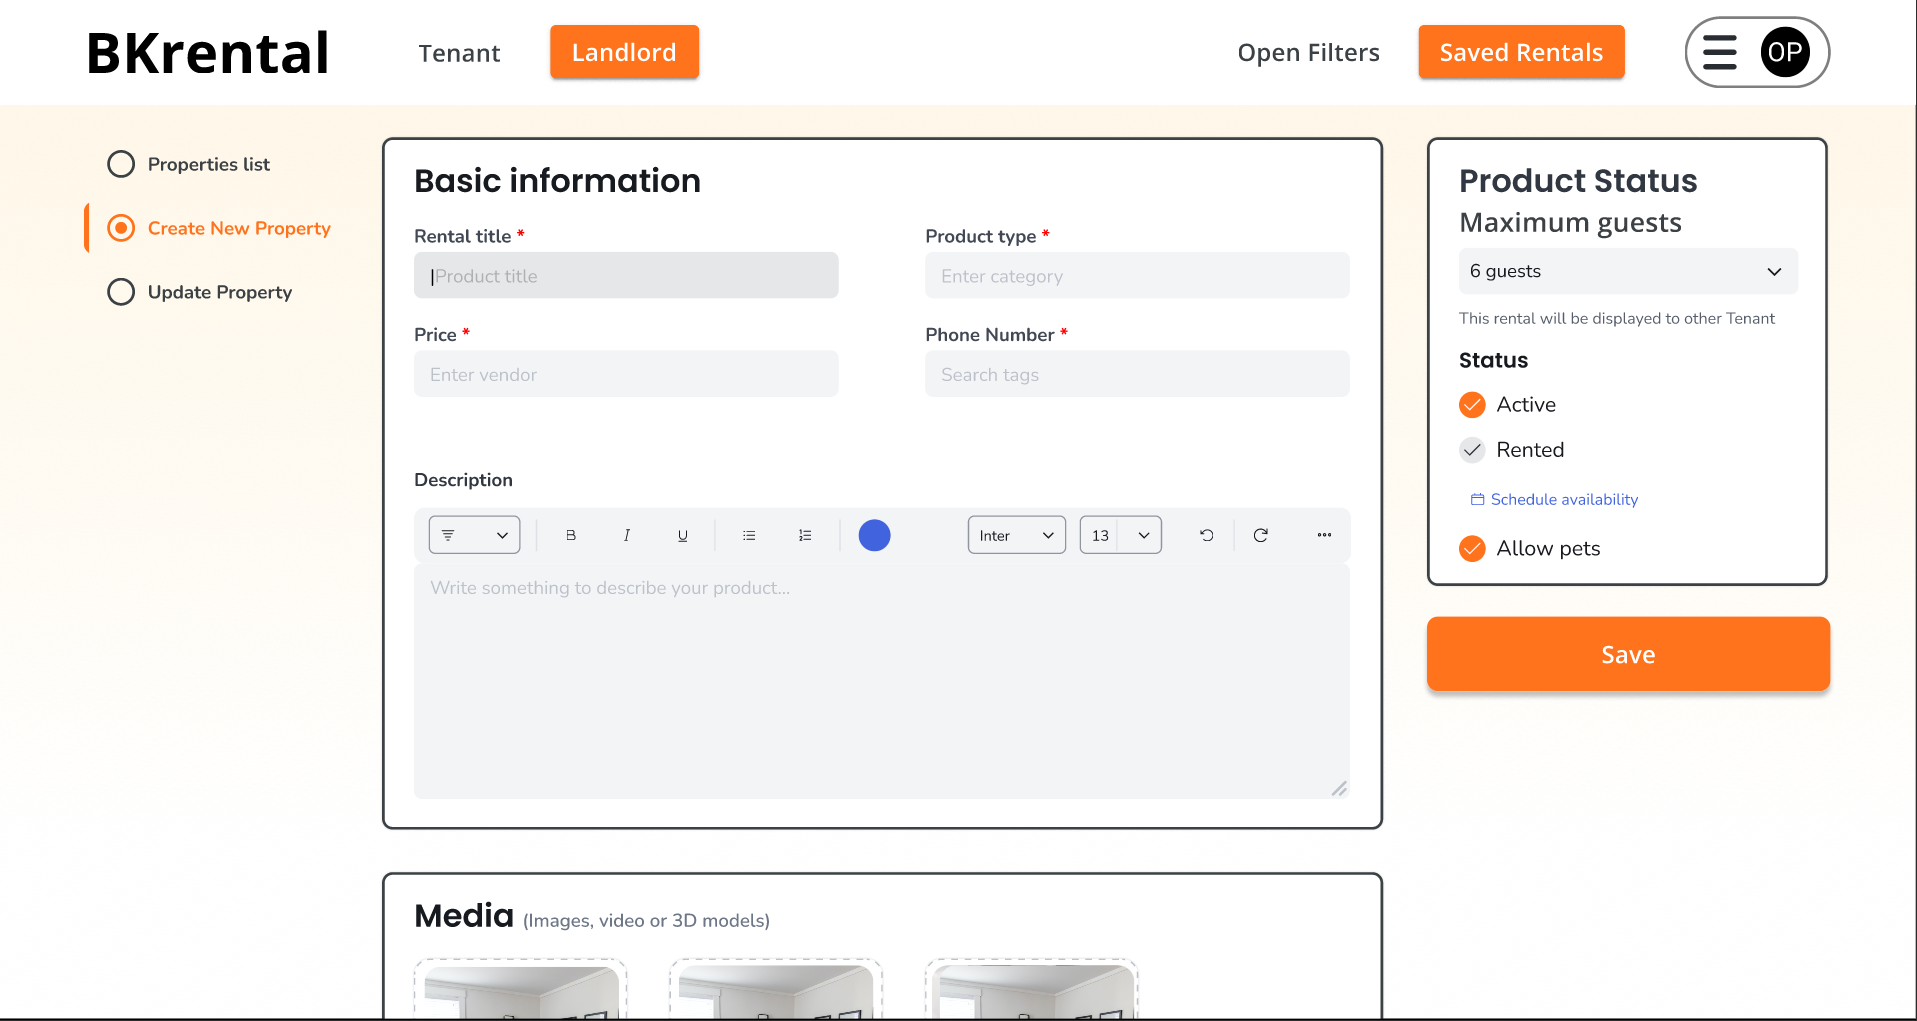
\includegraphics[width=0.8\textwidth]{Images/Mockup/create_rental_1.png}
    \caption{The form for the landlord to create a new rental post}
    \label{fig:create-rental-1}
\end{figure}

\begin{figure}[ht]
    \centering
    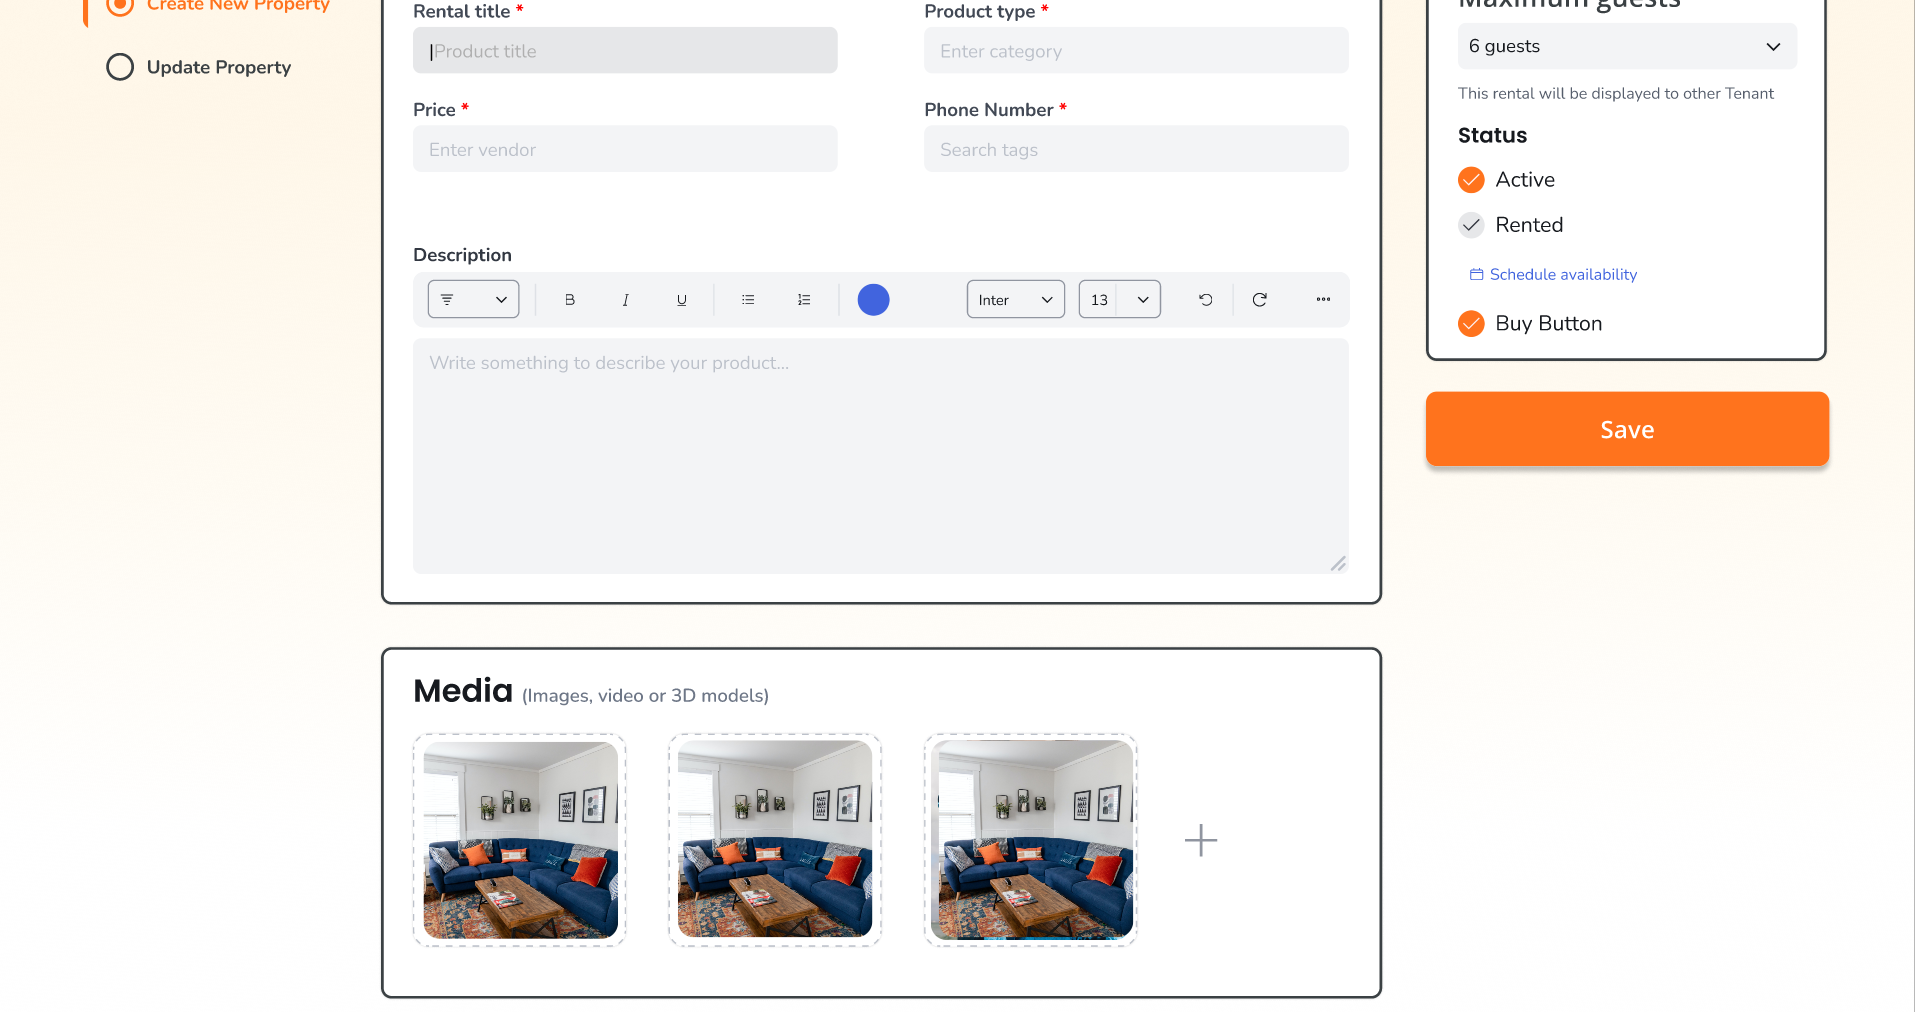
\includegraphics[width=0.8\textwidth]{Images/Mockup/create_rental_2.png}
    \caption{The form for the landlord to create a new rental post (continue)}
    \label{fig:create-rental-2}
\end{figure}

\clearpage

\begin{figure}[ht]
    \centering
    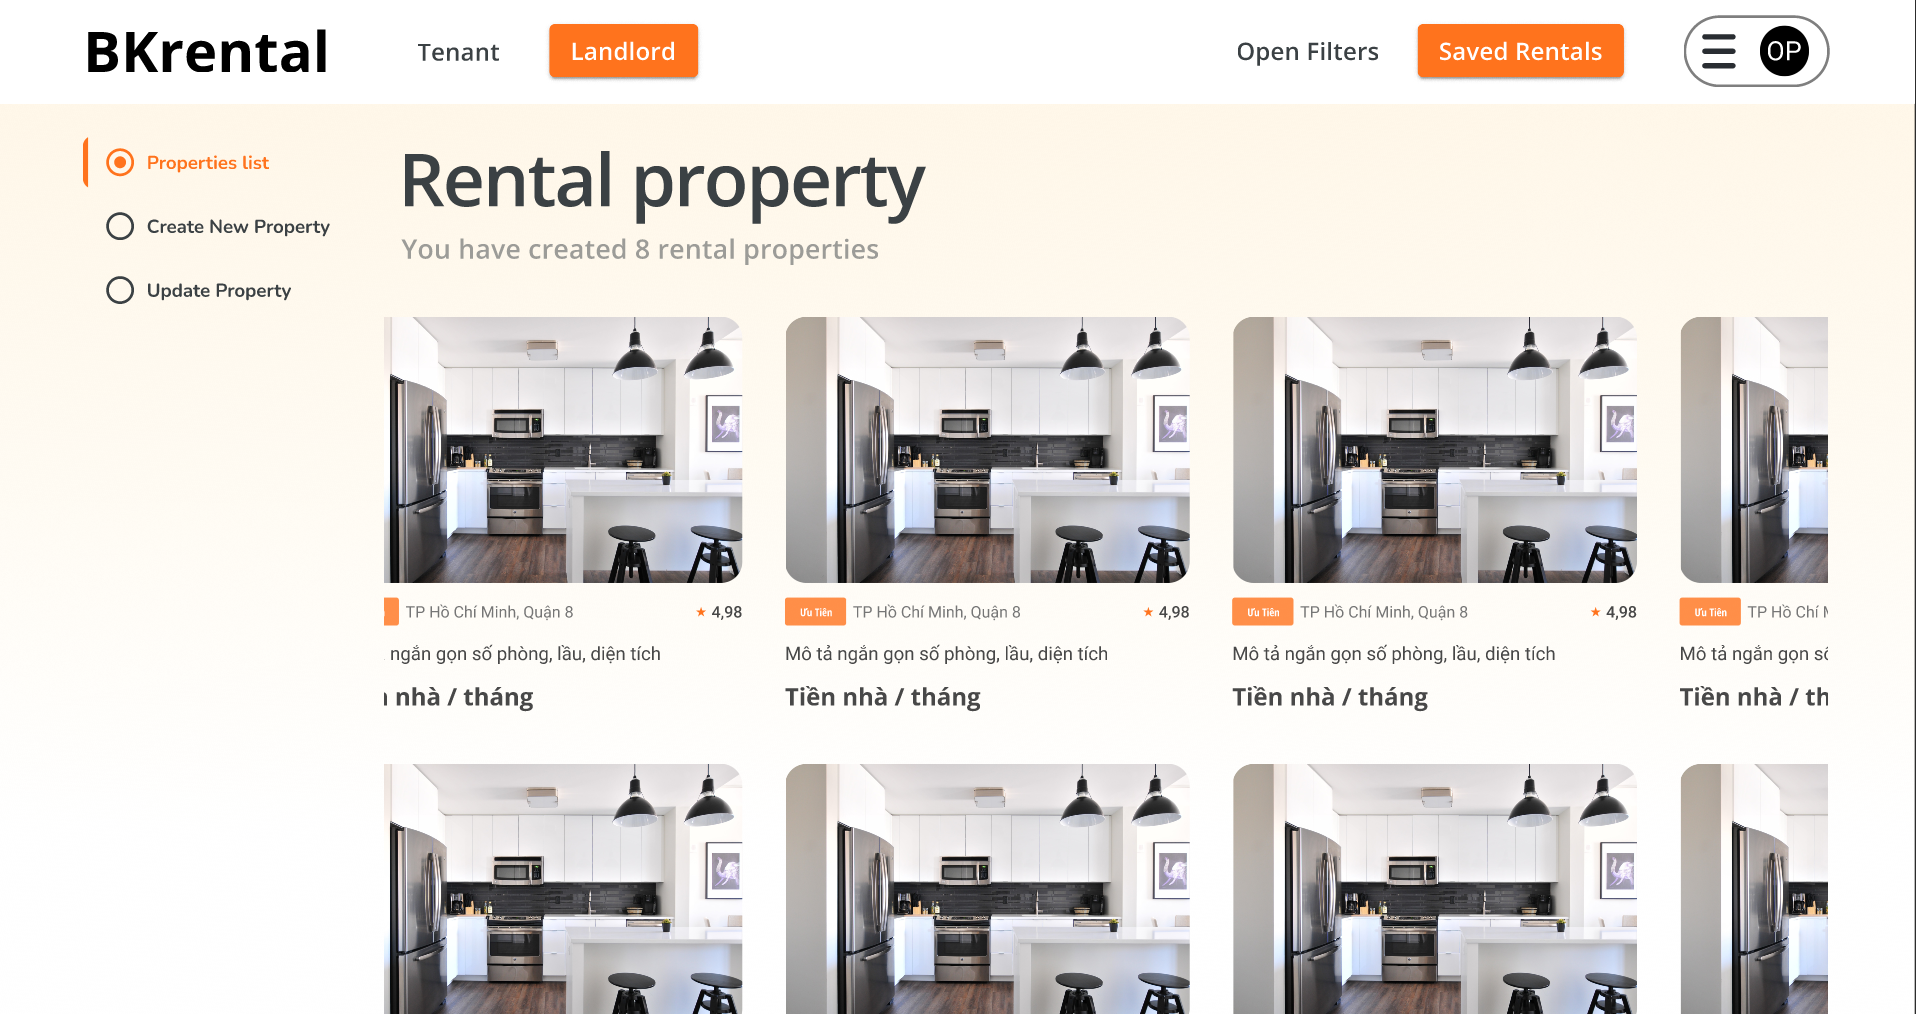
\includegraphics[width=0.8\textwidth]{Images/Mockup/property_list.png}
    \caption{The list of Landlords' properties}
    \label{fig:property_list}
\end{figure}

\begin{figure}[ht]
    \centering
    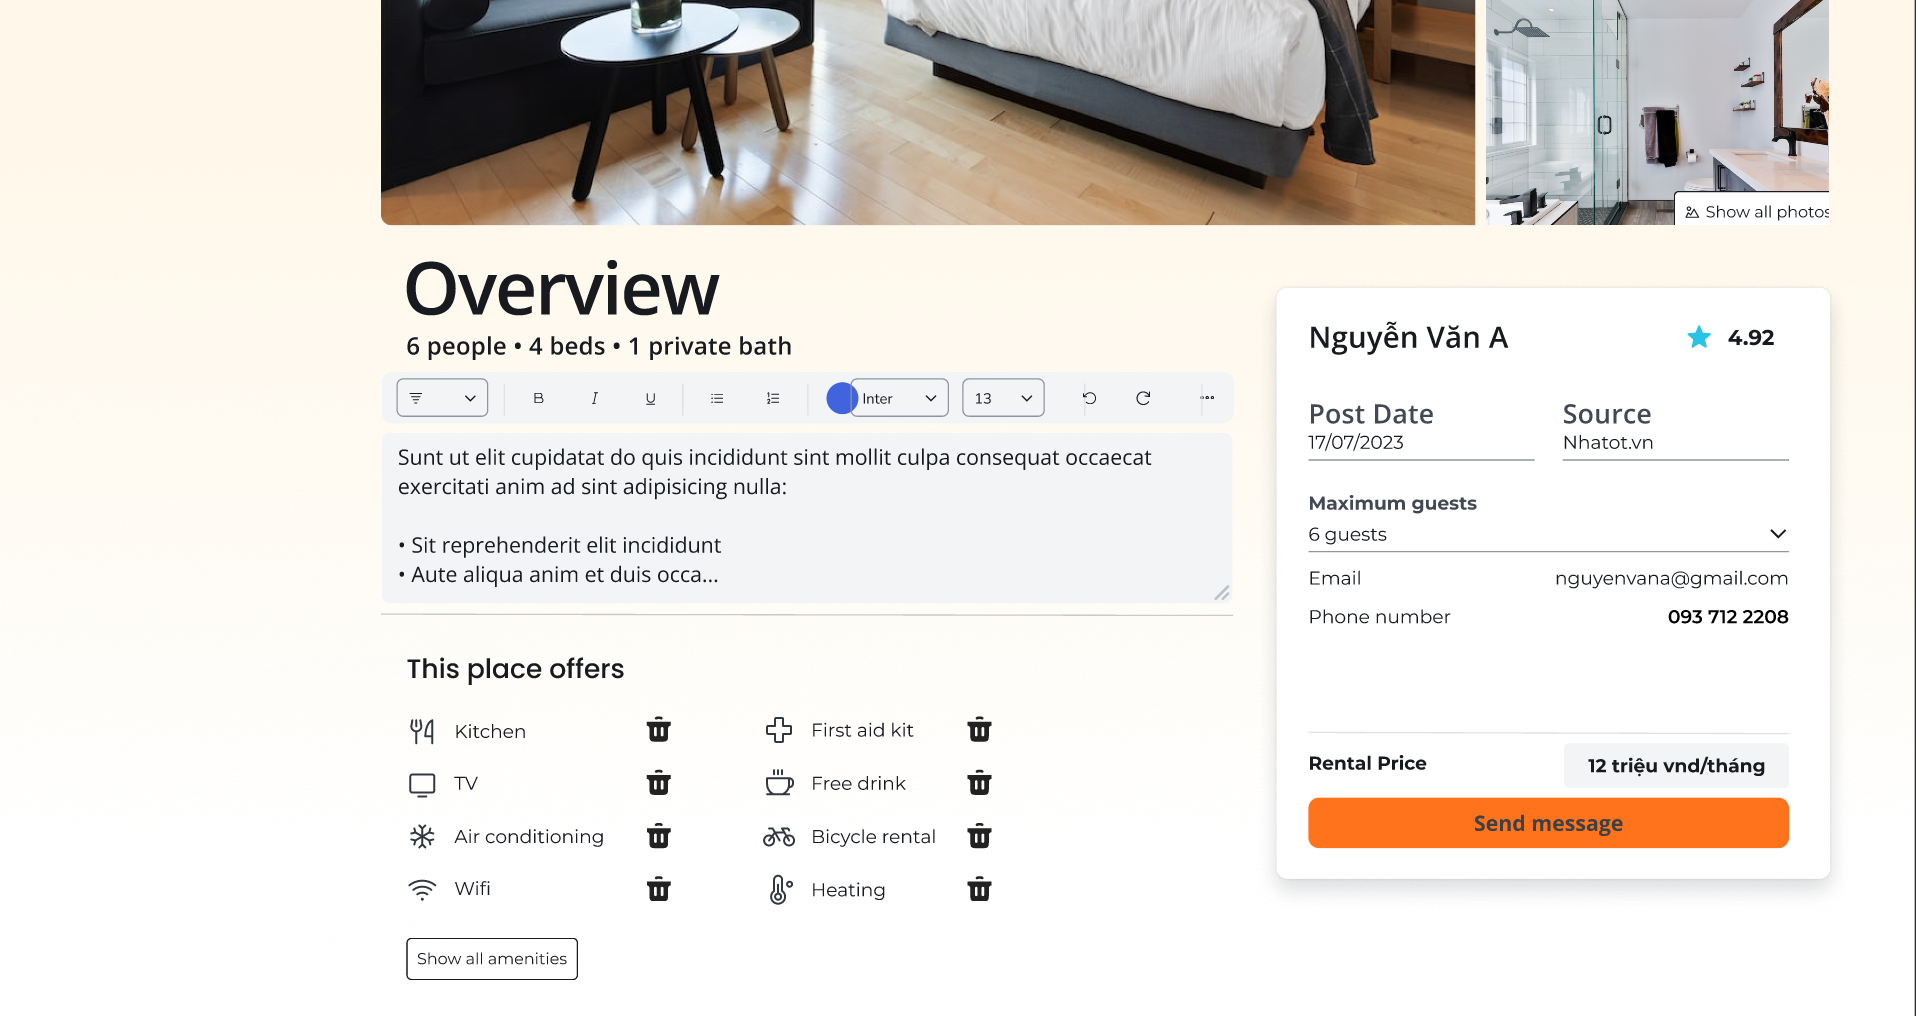
\includegraphics[width=0.8\textwidth]{Images/Mockup/update_rental.png}
    \caption{The form for the landlord to update a rental post}
    \label{fig:update_rental}
\end{figure}


\section{Crawler service}

\subsection{The Facebook Crawler}
We developed a tool that receives the list of Facebook pages and group URLs as input. Then this tool will get all the posts from these pages and groups and store them in the output file. The tool is implemented using NodeJS and the Puppeteer library.

We chose the list of 40 Facebook pages and groups in the real estate domain, especially the ones that have the most interactions. The list of these pages and groups is stored in the input file. The sample of the input file is shown in Figure \ref{fig:facebook-crawler-input}.

\begin{figure}[ht]
    \centering
    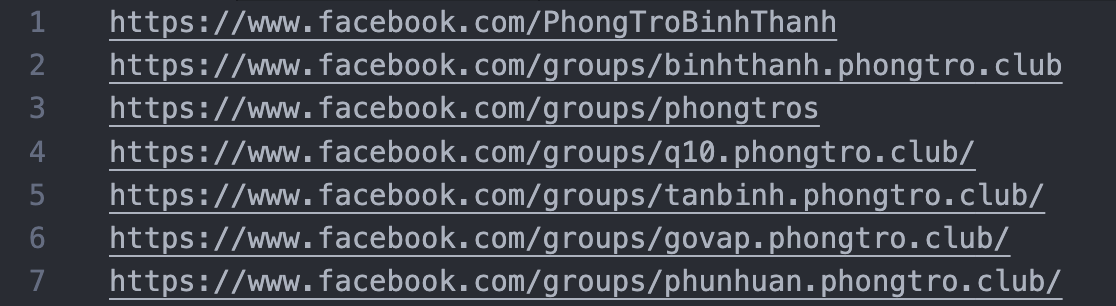
\includegraphics[width=0.8\textwidth]{Images/9.Implementation/facebook_crawler_input.png}
    \caption{The sample input of the Facebook crawler}
    \label{fig:facebook-crawler-input}
\end{figure}

When running the tool, the tool will read the input file and get the list of Facebook pages and groups. Then it will open a new browser window and log in to Facebook. After that, it will visit each page and group in the list and get all the posts from these pages and groups. Finally, it will store the posts in the output file. The output file is a text file that contains the list of posts in text format. Each post is separated by a new line character. After the tool finishes crawling all the posts, we get the output file that contains nearly \textbf{2000 posts}. The sample output of the tool is shown in Figure \ref{fig:facebook-crawler}.

\begin{figure}[ht]
    \centering
    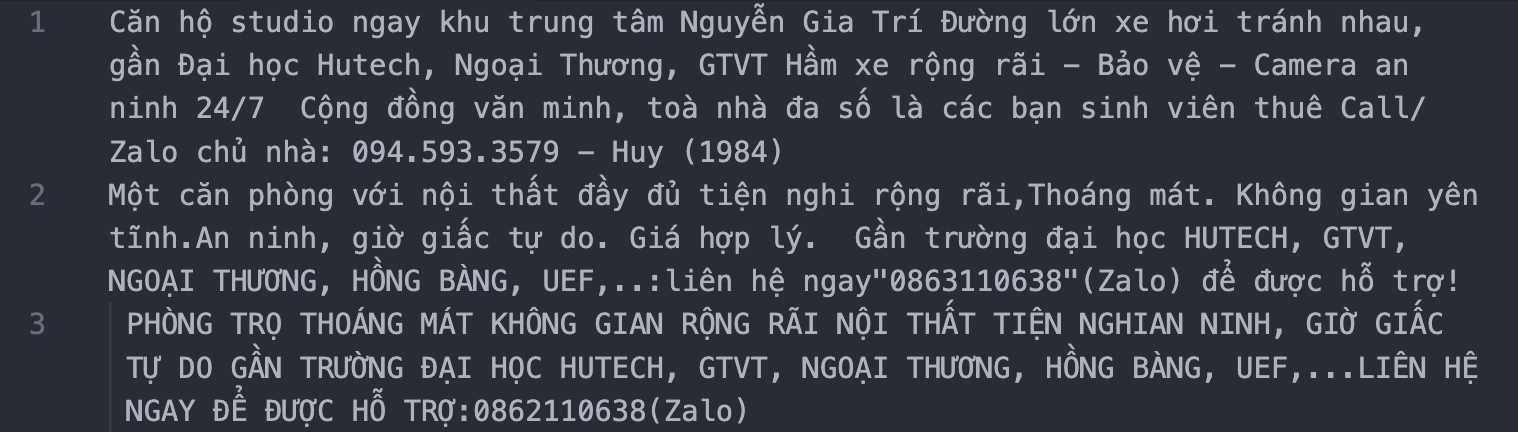
\includegraphics[width=0.8\textwidth]{Images/9.Implementation/facebook_crawler_output.png}
    \caption{The sample output of the Facebook crawler}
    \label{fig:facebook-crawler}
\end{figure}

\subsection{The Real Estate Website Crawler}
We also developed a tool that crawls the data from some popular real estate websites in Vietnam such as mogi.vn. The tool is implemented using Python and Scrapy. Because these websites are server-side rendered websites, we can take advantage of the Scrapy library to crawl the data. 

From the website link, we developed a Spider Scrapy. The main role of the Spider is downloading the content of the website parsing the content and getting the data by using CSS selector. The sample code of the parser is shown below

\begin{lstlisting}[language=Python]
def parse_detail_info(self, response):
    general_info = response.css('div.main-info')
    main_info = response.css('div.info-attrs.clearfix > *')
    agent_name_link = response.css('div.agent-name::text').get()
    agent_name_no_link = response.css('div.agent-name a::text').get()
    agent_name = agent_name_link if agent_name_link else agent_name_no_link

    yield rental_item = {
        'name': general_info.css('div.title h1::text').get(),
        'address': general_info.css('div.address::text').get(),
        'price': general_info.css('div.price::text').get(),
        'area': main_info[0].css('span:nth-of-type(2)::text').get(),
        'description': response.css('div.info-content-body').get(),
        'owner_name': agent_name,
        'owner_contact': response.css('div.agent-contact').get(),
        'post_date': main_info[2].css('span:nth-of-type(2)::text').get(),
        'prop_info_url': response.meta.get('prop_info_url')
    }
\end{lstlisting}

\section{Intent classification model}
We have implemented the intent classification model as discussed in \ref{sec:intent-classification-model} with Pytorch and PhoBERT library. The model is trained on the dataset containing 1000 labeled messages. We split the dataset into 2 parts: 80\% for training and 20\% for testing. We trained the model for 10 epochs with a batch size of 32. Figure \ref{fig:intent-classification-result} shows the accuracy of the model during the training process. Overall, the model achieves an accuracy of 97.4\% on the training set and 96.5\% on the test set. 

\begin{figure}[ht]
    \centering
    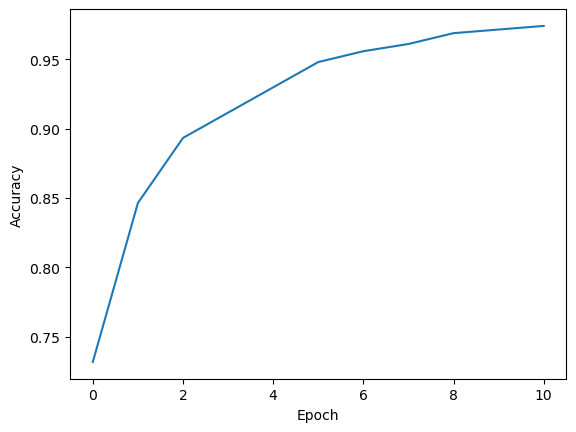
\includegraphics[width=0.8\textwidth]{Images/9.Implementation/intent_classifier_accuracy.png} 
    \caption{The accuracy of the intent classification model during the training process}
    \label{fig:intent-classification-accuracy}
\end{figure}

\begin{figure}[ht]
    \centering
    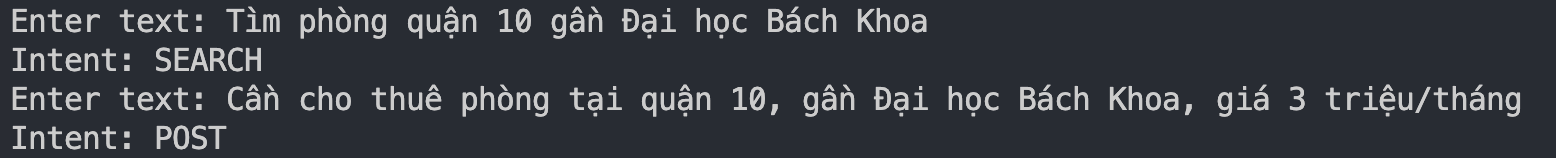
\includegraphics[width=0.8\textwidth]{Images/9.Implementation/intent_classifier_result.png}
    \caption{The sample result of intent classification model}
    \label{fig:intent-classification-result}
\end{figure}
